\documentclass[12pt,preprint]{aastex}
\usepackage{url}
\usepackage{natbib}
\usepackage{graphicx}
%\usepackage{subfig}
%\usepackage{fixltx2e}

%%%%%%%%%%%%%%%%%%%%%%%%%%%%%%%%%%%%%%%%%%%%%%%%%%%%
%%% author-defined commands
\newcommand\x         {\hbox{$\times$}}
\def\mic              {\hbox{$\mu{\rm m}$}}
\def\about            {\hbox{$\sim$}}
\def\Mo               {\hbox{$M_{\odot}$}}
\def\Lo               {\hbox{$L_{\odot}$}}

%\captionsetup[figure]{labelformat=simple}
%%%%%%%%%%%%%%%%%%%%%%%%%%%%%%%%%%%%%%%%%%%%%%%%%%%%

% Abstract

% Role of MOPS
% - Inputs and Responsibilities of MOPS : generating the Moving Objects table
% - Uses of Moving Objects table: Association and Science Users

% MOPS Functionality
% - SW standards/implementation status
% - Overview of history/refs (PS-MOPS, IOD)

% MOPS Sky-Plane Tracking:
% - Overview of system (tracklets, tracks, sky-plane tracking)
% - FindTracklets and algorithms
% - Tracklet Optimizations (collapseTracklets, subset removal) 
% - Metrics and graphs of SSM distributions in velocity
% - LinkTracklets (Kubica Algorithm) 
% - Track Filters (chi-squared, subset removal)
% - Metrics and graphs of SSM distributions in acceleration + velocity
% - IOD references



\begin{document}

\title{Moving Object Pipeline Requirements}

\author{}

\begin{abstract}

The Moving Object Pipeline System (MOPS) has two responsibilities
within LSST Data Management.  First, it is responsible for generating
and managing the \textbf{Moving Object} data products.  The Moving
Objects are identified solar system objects (SSOs) with associated
Keplerian orbits, errors, and a detected sources assocated with those
solar system objects.  The second responsibility of the MOPS is to
predict future locations of moving objects in incoming images so that
their sources may be associated with known objects; this will reduce
the number of transient detections and prevent Alert Generation for
known Solar System objects.

\end{abstract}

\tableofcontents

%\section{Science Requirements}

\section{System Design and Responsibilities}

The Moving Object Pipeline System has two main responsibilities: the
generation and maintenance of the Moving Object database, and the
prediction of known object locations which are sent to the Association
Pipeline to prevent unneccessary alerts.  In order to fulfill these
goals, the MOPS has been broken into several componenets, colloquially
known as ``DayMOPS'' and ``NightMOPS.''
 

\begin{figure}[!ht]
\begin{center}
  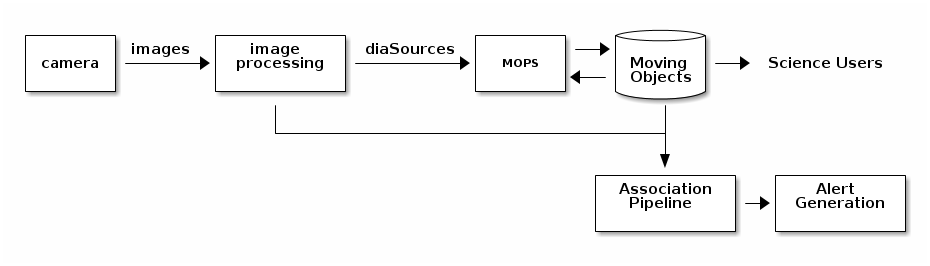
\includegraphics[width=13cm]{illustrations/mopsWithinLsst.png}
\end{center}
\caption{ Data flow from the camera through DayMOPS to the Science
  Users and Alert Generation.  DayMOPS will build and maintain the
  Moving Objects table, NightMOPS will use the Moving Objects table to
  communicate with the Assocation Pipeline.  }
\label{mopsWithinLsst}
\end{figure}


``DayMOPS,'' so called because it processes data acquired from the
previous night in a large batch operation, is responsible for
discovering new Moving Objects in newly-acquired data, searching old
data for detections of new objects, and updating the Moving Objects
table to reflect newly-acquired data. It is also responsible for
periodically cleaning and refining the contents of the Moving Objects
table.

``NightMOPS'' is responsible for projecting the locations of known
Moving Objects in upcoming images as they are announced during
night-time operations.  If Moving Objects are observed in these
images, then the Moving Object table is modified to add these
newly-acquired detections to their associated Moving Object.

The relationship between DayMOPS, NightMOPS and the neighboring
components of the LSST Data Management system is illustrated in
figure \ref{mopsWithinLsst}.

\subsection{DayMOPS: Discovering and Managing Moving Objects}

% Illustration of DayMOPS

% sky-plane vs. orbit-space illustration

The initial task of DayMOPS is to identify unknown objects present in
images and their orbits.  To accomplish this, the system initially
finds sets of detections which follow a sky-plane path roughly
consistent with asteroid motion; these sets of detections and their
fitted paths are called \textbf{tracks}.  This same method is the
basis for asteroid discovery used in the PanSTARRS Moving Object
Pipeline System \citep{psMOPSDesign}.  A set of algorithms for the
discovery of sky-plane tracks in dense data are presented in
\citet{Kubica:2005:MTA:1081870.1081889}; these algorithms are used in
the PanSTARRS MOPS as well.  Because of the loose approximations used,
many of the tracks will be mislinkages, combining detections which are
not attributable to the same source, but virtually all objects for
which a true (correctly-linked) track could be generated will get some
correct track.  LSST Data Management has developed additional
processing phases and filters which can improve the performance of the
system and reduce the computational costs by managing the number of
untrue or redundant tracks throughout the various phases of
processing.

Once tracks are discovered, they are sent to the Orbit Determination
phase. The Orbit Determination phase takes these sets of sky-plane
detections and attempts to find a Kepler orbit which could generate
the detections, if any exists.  This orbit is further refined, and
error bounds are established, using least-squares linearization.
Orbit Determination will reject many tracks as false, but should
successfully find fairly precise orbits for virtually all correctly
linked tracks.  Several methods for performing this task are known,
and several have implementations available to LSST
\citep{Milani04orbitdetermination}, \citep{Milani2006},
\citep{OpenOrb2009}, \citep{granvik_thesis}.  These orbits, and the
detections present in the track associated with that orbit, are used
to generate new Moving Objects.

\begin{figure}[h]
\begin{center}
  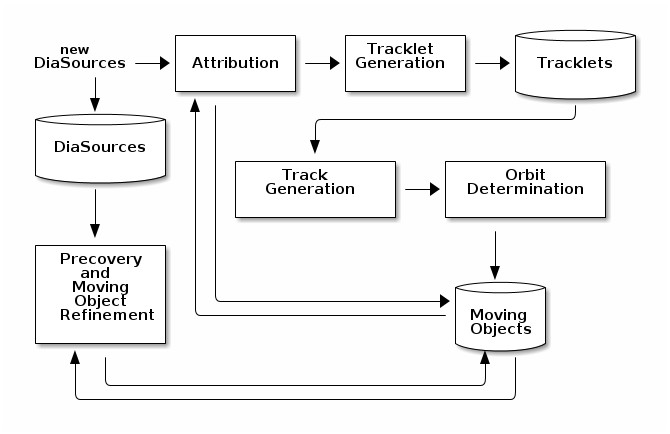
\includegraphics[width=11cm]{illustrations/mopsDiagram.png}
\end{center}
\caption{ Data flows into the DayMOPS pipeline and results in
  modifications of the Moving Objects table in a variety of ways,
  including attribution to known objects, a multi-stage pipeline for
  the discovery of new objects, and periodic refinements of the Moving
  Object table, such as possible merges of redundant objects or
  removal of false orbits. }
\label{mopsDiagram}
\end{figure}



As in the PanSTARRS MOPS design \citep{psMOPSDesign} the LSST's
DayMOPS is expected to perform several additional tasks to manage and
improve the Moving Objects table over time.  Attribution is the
process of identifying known objects in incoming data and adding those
detections to the correct Moving Object (this task is delegated to
NightMOPS). Similarly, Precovery is the recovery of known,
unattributed detections associated with a newly-discovered Moving
Object.  Another refinement is the merging of potentially redundant
Moving Objects.  The complete set of DayMOPS tasks and their data
flows are illustrated in figure \ref{mopsDiagram}.



\subsubsection{Building Tracklets}

% possible illustration: show Dec/time for two images, then tracklets in Dec/time

\textbf{Tracklets} are the building blocks of the sky-plane
\textbf{tracks} used by DayMOPS.  Tracklets are linkages between
DiaSource detections occuring within the same night; during this time
period, solar system object motion is linear or near-linear on the
sky. By creating tracklets, DayMOPS can find sky-plane position and
velocity estimates for sets of detections which may belong to solar
system objects.  This filters out many detections of non-solar system
objects, as they are less likely to generate tracklets.  The use of
tracklets also simplifies the downstream work of track generation,
which attempts to find sets of detections with a good
position/velocity/acceleration fit on the sky-plane; since tracklets
have known position and velocity, the track generation phase needs
only to find those tracklets compatible within some acceleration
factor.

In order to ensure that tracklet-generating images are acquired, it is
necessary to ensure that regions of the sky is visited two or more
times within an accepted time period within a night.  Currently, we
require that sky fields be revisited within a fairly short time period
($\leq 90$ minutes is the current rule) in order to constrain the
maximum apparent motion of solar system objects and thus also
constrain the number of tracklets.

The discovery of tracklets can be accomplished efficiently using
KD-Tree structures \citep{bentley_kdtrees} and methods from
\citet{kubica_thesis}.  DayMOPS will build one (RA, Dec) KD-Tree for
each image, holding the detections found in that image.  Because
KD-Trees allow quick range searches of arbitrary-dimensional spatial
data, it is possible to efficiently perform searches over the
detections to find pairs of detections sufficiently close within time
and within limits on apparent velocity. These pairs of detections are
linked to generate tracklets.
% TBD: Is this clear?!

% psuedo code?

Further refinements of tracklets are possible with additional
processing. If an object gets more than one tracklet, it is possible
to use methods similar to the Hough transform (CITE HOUGH, SELF) to
identify and merge these redundant tracklets into larger tracklets,
improving the linear position/velocity fits of the tracklets and
reducing the number of tracklets passed downstream.

\subsubsection{Building Tracks}

Over the course of roughly one month, solar system objects tend to
follow a roughly quadratic path on the sky-plane
\citep{kubica_thesis}.  The track generation phase of DayMOPS will
attempt to find sets of tracklets (which have position and velocity
estimates) which were observed within one month of each other and are
compatible within some sky-plane acceleration factor.  Tracks which
are suitable for generating a reasonable orbital fit are sent to the
Orbit Determination phase. 

The methods used for tracklet-to-tracklet linking are described in
\citet{kubica_thesis} and \citet{Kubica:2005:MTA:1081870.1081889}.
The methods described attempt to efficiently find sets of tracklets
which are \textit{compatible} in the sense that they could be joined
to form a track: that is, tracklets which span multiple nights and
have positions and velocities which are consistent with a fixed
acceleration.  

To perform this work efficiently, these methods use four-dimensional
KD-Trees over \textit{tracklets-space}, or (RA position, Dec position,
RA velocity, Dec velocity). One tree is created per image, and holds
each tracklet which has its first detection in that image.  A
multi-tree walk is performed using a clever algorithm, efficiently
discovering all regions of tracklet-space which could contain sets of
tracklets that are compatible, while avoiding visits to tracklet-space
regions which are not compatible and could not generate a track.  This
is performed recursively until leaf nodes of the KD-Trees are reached.

% illustration from Kubica?

When the algorithm encounters a set of leaf nodes in the KD-Trees, it
attempts to build a track using the detections held in the tracklets
at the leaf nodes.  A quadratic fit, or if possible, a higher-order
fit, to the day will be attempted.  Then a quality-of-fit assessment
is used to determine whether the track is considered acceptably
credible to pass downstream to the Orbit Determination.  Investigation
into ideal quality-of-fit metrics is ongoing, but as of this writing a
filter on minimum chi-squared probability appears to be the best
option.



\subsection{NightMOPS: Predicting Moving Object Locations}

The NightMOPS section of MOPS is responsible for predicting the
locations of known Moving Objects as images are taken, so that they
may be attributed to the known Moving Objects and removed from the set
of unknown transients detections.  This allows attribution for known
Moving Objects, improving the quality of the Moving Object data
products, and also allows the prevention of unnecessary Alerts.

Predicting the locations of objects given an orbit can be accomplished
through ephemeris calculation using existing orbit-space software
suites \citep{Milani2006}, \citep{OpenOrb2009}.  However, ephemeris
calculation can be fairly slow due for large data sets.  Because the
observations schedule for LSST will be determined dynamically, it is
necessary to generate ephemeris predictions for a large Moving Object
table in a short period of time.

% some kind of time-domain illustration?

In order to accomplish this, NightMOPS will generate ``coarse
ephemerides'' for known objects, predicting their locations at the
beginning and end of the night.  Then, when given an upcoming image
location, NightMOPS will use interpolation of the coarse ephemerides
to find objects which could feasibly be present in the upcoming
image. Precise ephemerides for just these objects will be
generated. In this way, NightMOPS will avoid the problem of generating
ephemeris for each known Moving Object for every image time.


\subsection{Implementation Status}

All software components of MOPS, with the possible exception of
initial orbit determination, and orbital least-squares linearization
fitting of orbits to data, and ephemeris generation, is expected to be
completed in open-source C++ compliant with LSST software guidelines
and in LSST appropriate coding style.  These components will run
inside the LSST Pipeline Framework.  

Currently, the initial tracking phases of DayMOPS are implemented in
LSST-compliant C++.  The selection of an appropriate package for
initial orbit determination, least-squares linearization of orbit
fitting, and ephemeris generation is incomplete but several FORTRAN
options are available to us, some open-source.  A Python-based
implementation of NightMOPS, using the LSST Pipeline Framework, is
complete but it is currently using a closed-source ephemeris
generation tool.




\section{MOPS Metrics \& Scaling}



\section{Development Plan}



\bibliographystyle{apj}
\bibliography{baseline}

\end{document}
